%   Filename    : chapter_3.tex 
\chapter{Research Methodology}
This chapter lists and discusses the specific steps and activities that will be performed to accomplish the project. 
The discussion covers the activities from pre-proposal to Final SP Writing.

\section{Development Process/Design of Study }
ISay is a system website to be prototyped according to the needs of the UPV guidance counselors which is to make their services available online and to the needs of UPV students which is to avail guidance and counseling services with ease of access. This system website will include functions for the administrators and clients. 

\begin{table}   %t means place on top, replace with b if you want to place at the bottom
\centering
\caption{For registered UPV guidance counselors:} \vspace{0.25em}
\begin{tabular}{|p{2in}|p{4in}|} \hline
\centering Functions & Descriptions\\ \hline
Create an Account       &    For UPV guidance counselors, to create an ISay account is to enable them to be able to do the other functions intended for them. \\ \hline
Login to Account  &  To login into the system as guidance counselors and administrator.\\ \hline
Manage Pending Appointments for Approval  & UPV guidance counselors will be able to view pending appointments for approval and manage them properly. \\ \hline
Direct Message a Registered User (Student)       &    UPV guidance counselors will be able to contact registered users (students) within ISay.  \\ \hline
Summarize Records & UPV guidance counselors will be able to summarize records kept after each appointment according to demographic details for a week, a month, or a year. \\ \hline
\end{tabular}
\label{tab:registeredcounselors}
\end{table}

\begin{itemize}
\item For registered UPV guidance counselors, see \ref{tab:registeredcounselors}
\item For registered UPV student users, see \ref{tab:registeredstudents}
\end{itemize}

\begin{table}   %t means place on top, replace with b if you want to place at the bottom
\centering
\caption{For registered UPV student users:} \vspace{0.25em}
\begin{tabular}{|p{2in}|p{4in}|} \hline
\centering Functions & Descriptions\\ \hline
Create an Account       &   For UPV students, to create an ISay account is to enable them to inquire about services, book appointments, and direct message a guidance counselor.  \\ \hline
Login to Account  &  To login into the system as a registered user. \\ \hline
Select Services   & UPV students will be able to view available services on the homepage of the ISay.  \\ \hline
Direct Message a Guidance Counselor       &    UPV students will be able to contact registered guidance counselors within ISay to ask for additional inquiries without leaving the website.   \\ \hline
Schedule an Appointment  & UPV students will be able to book an appointment for the service they would like to avail of according to their preferred available time, date, and mode of communication.  \\ \hline
\end{tabular}
\label{tab:registeredstudents}
\end{table}


According to Kumar et al (2012), the use of agile methodologies has an advantage to productivity and quality. As it has different types such as Extreme Programming, Scrum, Feature Driven Development (FDD), and Crystal Method. For this study, there will be no specific type of agile methodology to be used. Instead, backend and frontend programming will be done alongside testing to ensure the development quality. The product will be shown to the UPV Guidance and Counseling if all the aforementioned functions are done at the end of the school year. 


\section{Persons Involved}
 The following are the persons involved in the development of ISay: 
	\begin{itemize}
	\item UPV Guidance and Counseling Unit Resource Person. The resource person is contacted before the planning started to pitch-in the idea of the system website. This is because the programmers and researchers would like to know comments and suggestions of how the service unit will use the system website if a system website will be made. 
	\item  Adviser. The adviser will be the person who will help both the programmers and researchers during the development of the system website. 
	\item Programmers. The programmers are students who have knowledge in backend and frontend programming that will be used in order to develop the system website. 
	\item  Researchers. The researchers are students who will be responsible for the activities that include inquiry, research, brainstorming, consultation, and documentation. 
	\end{itemize}


\section{Tools/Technical and Software Specification}
The following are the tools that will be used in order to develop ISay: 
	\begin{itemize}
	\item Django. This high-level Python web framework is used if developers want to rapidly develop a clean and pragmatic design. This is free and open source.
	\item  HTML. This is a markup language that shapes the structure of web content. This is consists of elements, which are used to enclose or wrap the different parts of web content to make it appear or act in a specific manner. 
	\item Windows Operating System.  
	\item  TexStudio and Microsoft Word (documentation) 
	\item Dia (diagrams) 
	\item Zoom (consultations and meetings with the adviser and resource person) 
	\item GitHub 
	\end{itemize}


\section{User Specifications}
	\begin{itemize}
	\item \textbf{UPV students.} They are primary users who will be called clients. Clients will have their own account to enable functions such as inquiring, scheduling of appointments, and direct messaging a guidance counselor within the website. 
	\item \textbf{Guidance Counselors.} They are the other primary users and can, also, be called administrators since they will be the ones managing appointments and summarizing records. 
	\item \textbf{Adviser.} The adviser is the one who will supervise the development of the ISay, thus he is one of the people that will probably use ISay. 
	\item \textbf{Programmers.} They will be the one making ISay, and to use ISay is to test its quality every incremental development. 
	\end{itemize}

\section{Assumptions and Dependencies}
ISay is dependent on the guidance counselors, as well as the services they provide. Thus, without guidance counselors/administrators, there will be no services supplied which in turn no UPV students will sign up to ISay. 

\section{Apportioning of Requirements}
If the development of ISay comes to a delay, major requirements should be prioritized. 

\section{System Specifications}

\newpage
\subsection{Activity Diagrams}

\begin{figure}[h!]                %-- use [t] to place figure at top, [b] to place at the bottom, [h] for here
\centering                    %-- use this to center the figure
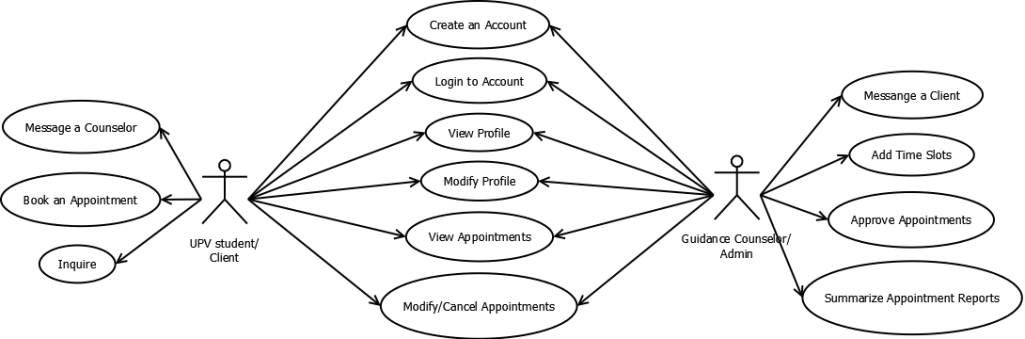
\includegraphics[width=\textwidth]{Activity_Diagram.png}     
\caption{Activity Diagram}
\label{fig:activitydiagram}
\end{figure}

\subsection{Functional Requirements}
	\begin{enumerate}
	\item User Specifications 
		\begin{itemize}
		\item REQ1. The system website should enable Clients and Admins to create an account. 
		\item REQ2. The system website should enable Clients and Admins to log in to their accounts. 
		\item REQ3. The system website should enable Clients and Admins to view their profile account. 
		\item REQ4. The system website should enable Clients and Admins to modify their profile account. 
		\item REQ5. The system website should enable Clients to message a guidance counselor/admin. 
		\item REQ6. The system website should enable Admins to message a UPV student/client.  
		\item REQ7. The system website should enable Clients to inquire about services. 
		\item REQ8. The system website should enable Admins to add timeslots. 
		\item REQ9. The system website should enable Clients to book an appointment. 
		\item REQ10. The system website should enable Admins to approve appointments. 
		\item REQ11. The system website should enable Clients and Admins to view their scheduled appointments. 
		\item REQ12. The system website should enable Clients and Admins to modify or cancel appointments. 
		\item REQ13. The system website should enable Admins to summarize appointment reports. 
		\item REQ14. The system website should enable Clients and Admins to log out of their accounts. 
		\end{itemize}

	\item System Requirements 
		\begin{itemize}
		\item The system website should enable Clients and Admins to create an account. 
			\begin{itemize}
			\item They shall provide their email address given by the school, full name, desired username, and create their password. 
			\item Check if the credentials given are valid: 
				\begin{itemize}
				\item The username is still available. 
				\item The password is not empty. 
				\item The password is the same as the confirm password. 
				\item The email address has not been used. 
				\end{itemize}
		\item If credentials are valid, save and add them to the database. 
		\end{itemize}

		\item The system website should enable Clients and Admins to login to their account. 
			\begin{itemize}
			\item They shall provide their username and password. 
			\item Check if credentials saved are the same as the ones provided. 
			\item Access shall be granted or denied. 
			\end{itemize}
		\item The system website should enable Clients and Admins to view their profile account. 
			\begin{itemize}
			\item The information saved should be displayed accordingly. 
			\end{itemize}
		\item The system website should enable Clients and Admins to modify their profile account. 
			\begin{itemize}
			\item They shall provide their new information. 
			\item The old information will be replaced by the new one in the database. 
			\end{itemize}
		\item The system website should enable Clients to message a guidance counselor/admin. 
			\begin{itemize}
			\item The system website shall require a message content from the client to send a message to the guidance counselor/admin. 
			\end{itemize}
		\item The system website should enable Admins to message a UPV student/client.  
			\begin{itemize}
			\item The system website shall require message content from the guidance counselor/admin to send a message to the client.  
			\end{itemize}
		\item The system website should enable Clients to inquire services. 
			\begin{itemize}
			\item The system website shall display service description. 
			\end{itemize}
		\item The system website should enable Admins to add timeslots. 
			\begin{itemize}
			\item The guidance counselor or administrator will provide the time he or she will be available. 
			\item The information will be saved to the database. 
			\end{itemize}
		\item The system website should enable Clients to book an appointment. 
			\begin{itemize}
			\item The system website shall check if the client is logged in or not. 
			\item The patient shall select the college and department he or she is enrolled in or hired. 
			\item The system website shall display the assigned guidance counselor(s) for that specific department, alongside his or her available time. 
			\item The system website shall generate a unique booking number for each appointment. 
			\item The system website shall send a notification email stating that approval from the guidance counselor is a must to confirm the appointment.  
			\end{itemize}
		\item The system website should enable Admins to approve appointments. 
			\begin{itemize}
			\item The system website shall display appointments waiting for approval. 
			\item If the guidance counselor has no prior unstated appointment, he or she shall approve the appointment. 
			\item The system website shall send a confirmation email to the client that the appointment is booked successfully. 
			\end{itemize}

		\item The system website should enable Clients and Admins to view their scheduled appointments. 
			\begin{itemize}
			\item The system website shall display the scheduled appointments of the clients and guidance counselors according to date. 
			\end{itemize}
		\item The system website should enable Clients and Admins to modify or cancel appointments. 
			\begin{itemize}
			\item The system website shall allow confirmed appointments to be modified without asking for the patient's information. 
			\item The system website shall only ask for the unique booking number. 
			\item The system website shall make necessary updates after the client’s or guidance counselor’s changes have been made. 
			\end{itemize}
		\item The system website should enable Admins to summarize appointment reports. 
			\begin{itemize}
			\item The system shall allow admins to manage and access database information accordingly. 
			\end{itemize}
		\item The system website should enable Clients and Admins to logout of their account. 
			\begin{itemize}
			\item Logout client or admin out of the system website when they click logout. 
			\end{itemize}
		\end{itemize}
	\end{enumerate}


\subsection{Non-Functional Requirements}
	\begin{enumerate}
	\item Performance
		\begin{itemize}
		\item The system website must have a good response time.
		\item The system website must run error while operating with a huge data set.  
		\end{itemize}
	\item Reliability
		\begin{itemize}
		\item The system website should be available when requested for service by clients and admins. 
		\end{itemize}
	\item Safety 
		\begin{itemize}
		\item The system website should maintain a good backup.  
		\end{itemize}
	\item Security
		\begin{itemize}
		\item External communications between the system website’s data servers, clients and admins must be encrypted. 
		\end{itemize}
	\item Supportability
		\begin{itemize}
		\item The system website should be able to be transferred from one environment to another. 
		\item The system website should be easy to maintain. 
		\item The system website should be able to deal with additional international conventions such as number formats, etc. 
		\item The system should be able to be used on multiple platforms.  
		\end{itemize}
	\item Usability
		\begin{itemize}
		\item The system website should have informative error messages. 
		\item The system website should be user-friendly. 
		\end{itemize}
	\end{enumerate}

\subsection{Sequence Diagrams}

\begin{figure}[!h]                %-- use [t] to place figure at top, [b] to place at the bottom, [h] for here
\centering                    %-- use this to center the figure
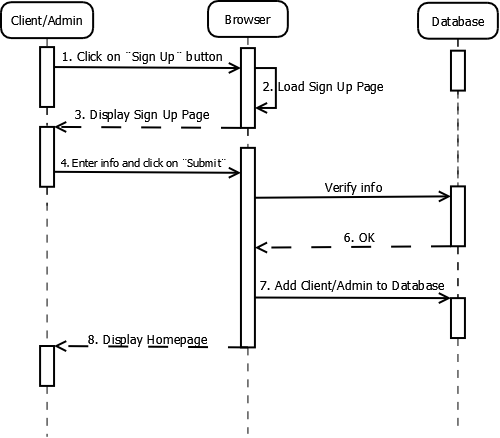
\includegraphics[width=\textwidth]{SignUp_SQ.png}     
\caption{Sequence diagram on Creating an Account }
\label{fig:createacctsq}
\end{figure}


\newpage
\begin{figure}[!h]                %-- use [t] to place figure at top, [b] to place at the bottom, [h] for here
\centering                    %-- use this to center the figure
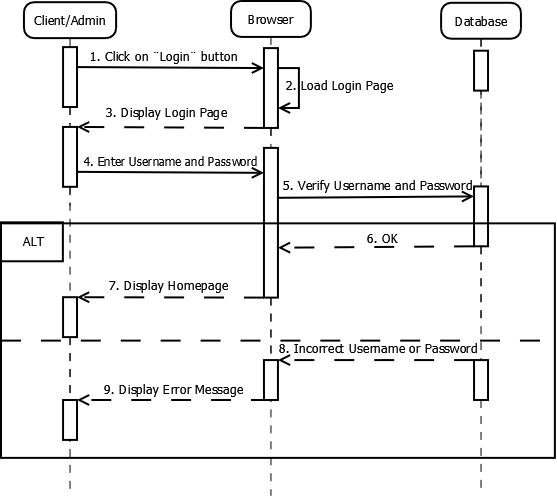
\includegraphics[width=\textwidth]{Login_SQ.png}     
\caption{Sequence diagram on Login }
\label{fig:loginsq}
\end{figure}

\newpage
\begin{figure}[!h]                %-- use [t] to place figure at top, [b] to place at the bottom, [h] for here
\centering                    %-- use this to center the figure
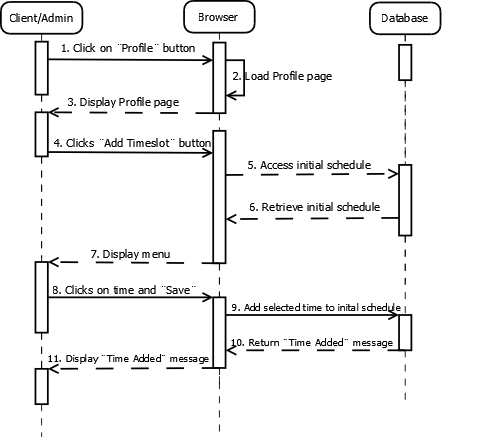
\includegraphics[width=\textwidth]{AddTimeslot_SQ.png}     
\caption{Sequence diagram on Add Timeslot }
\label{fig:timeslotsq}
\end{figure}

\newpage
\begin{figure}[!h]                %-- use [t] to place figure at top, [b] to place at the bottom, [h] for here
\centering                    %-- use this to center the figure
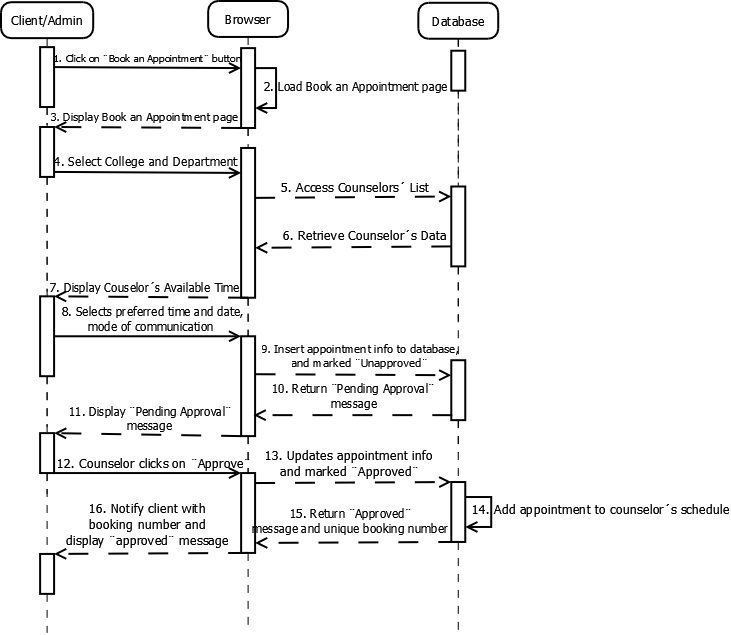
\includegraphics[width=\textwidth]{Book_SQ.png}     
\caption{Sequence diagram on Booking an Appointment }
\label{fig:bookappsq}
\end{figure}


\begin{figure}[!hp]                %-- use [t] to place figure at top, [b] to place at the bottom, [h] for here
\centering                    %-- use this to center the figure
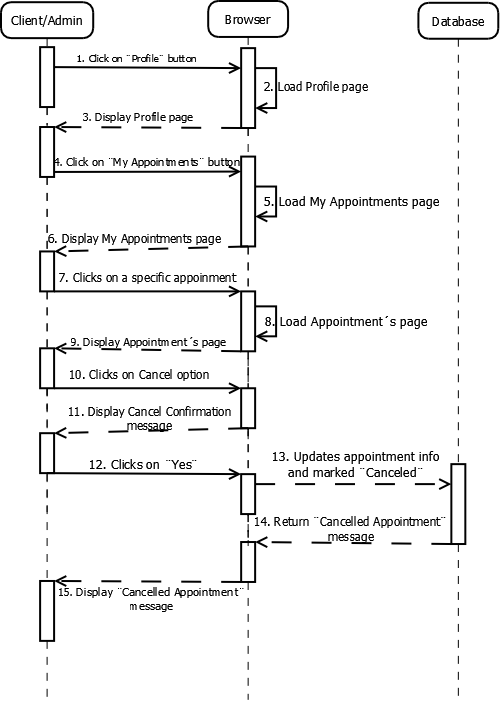
\includegraphics[width=\textwidth]{Cancel_SQ.png}     
\caption{Sequence diagram on Cancelling Appointment }
\label{fig:cancelsq}
\end{figure}


\begin{figure}[!hp]                %-- use [t] to place figure at top, [b] to place at the bottom, [h] for here
\centering                    %-- use this to center the figure
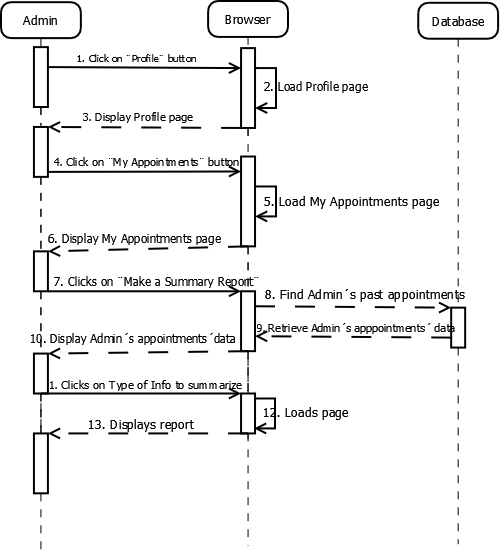
\includegraphics[width=\textwidth]{Report_SQ.png}     
\caption{Sequence Diagram on Summarizing Reports }
\label{fig:repsq}
\end{figure}


\newpage

\section{Procedures}
%\subsection{Detailed User Interface}


\subsection{Hardware Interface}
\begin{itemize}
\item Any mobile device 
	\begin{itemize}
	\item Requirements: 
		\begin{itemize}
		\item The mobile device should be charged enough to be able to connect to the Internet and finish an activity. 
		\item The mobile device should be connected to the Internet through a wired or wireless connection. 
		\end{itemize}
	\item Risks:
		\begin{itemize}
		\item If the device has insufficient charge and power interruption happens, unfinished activity might be expected. 
		\end{itemize}
	\end{itemize}
\item Internet Provider Devices 
	\begin{itemize}
	\item Requirements: 
		\begin{itemize}
		\item The Internet Provider device should be plugged into an electric provider for the device to function and connect to the Internet. 
		\item Data should be available to be able to connect to the Internet. 
		\end{itemize}
	\item Risks:
		\begin{itemize}
		\item If the device is connected to a public network and has no anti-virus software, the risk of being hacked has a higher probability. 
		\item Since most of the Internet Provider devices are power-dependent, the unavailability of electricity might result in unfinished activity. 
		\end{itemize}
	\end{itemize}
\end{itemize}

\newpage
\subsection{Testing (Procedure)}
This section will show the procedure that the programmers will be conducting every unit testing. 

\begin{table}[h!]   %t means place on top, replace with b if you want to place at the bottom
\centering
\caption{Test Case 1. Create an Account} \vspace{0.25em}
\begin{tabular}{|p{2in}|p{4in}|} \hline
\centering 
Test Case ID & TestCase-01 \\ \hline
Test Case Name       &   Create an Account   \\ \hline
Pass/Fail Criteria       &   The test passes if the client/admin provides information like school email address, full name, username, password, and confirm password.    \\ \hline
Input Data  &  Alphanumeric and characters key code  \\ \hline
Test Procedure   & Expected Outcome  \\ \hline
Step 1. Empty fields in the form.        &    An error message is displayed under the input fields.    \\ \hline
Step 2. Fill in all input fields.   & Check if password and confirm password are similar. If similar, email address string is checked if there’s a string “@up.edu.ph”. If email has the string and is not used by another client/admin, a new client/admin is created and added to the database.   \\ \hline
Step 3. Type unsimilar passwords in input fields, password and confirm password. & An error message is displayed under the input fields. \\ \hline
Step 4. Type similar passwords in input fields, password and confirm password. & If similar, email address string is checked if there’s a string “@up.edu.ph”. If email has the string and is not used by another client/admin, a new client/admin is created and added to the database.  \\ \hline
\end{tabular}
\label{tab:test1}
\end{table}

\newpage
\begin{table}[h!]   %t means place on top, replace with b if you want to place at the bottom
\centering
\caption{Test Case 2.  Login to Account} \vspace{0.25em}
\begin{tabular}{|p{2in}|p{4in}|} \hline
\centering 
Test Case ID & TestCase-02 \\ \hline
Test Case Name       &   Login to Account    \\ \hline
Pass/Fail Criteria       &   The test passes if the client/admin provides correct information like school email address/username, password.     \\ \hline
Input Data  &  Alphanumeric and characters key code  \\ \hline
Test Procedure   & Expected Outcome  \\ \hline
Step 1. Type an incorrect email address/username or password.         &    An error message is displayed under the input fields.    \\ \hline
Step 2. Type a correct email address/username or password.   & Client/admin is redirected to the homepage.     \\ \hline
\end{tabular}
\label{tab:test2}
\end{table}



\begin{table}[h!]   %t means place on top, replace with b if you want to place at the bottom
\centering
\caption{Test Case 3. Homepage} \vspace{0.25em}
\begin{tabular}{|p{2in}|p{4in}|} \hline
\centering 
Test Case ID & TestCase-03 \\ \hline
Test Case Name       &   Homepage     \\ \hline
Pass/Fail Criteria       &   The test passes if the website opens. This is the default page of the system website.      \\ \hline
Input Data  &  Enter the system website’s URL into the browser with an Internet connection.   \\ \hline
Test Procedure   & Expected Outcome  \\ \hline
Step 1. Click on any page links present on the page.         &   Redirects the client/admin to the page linked to that page link present on the homepage.     \\ \hline
Step 2. Click on the system website logo.    & 	Directs to the homepage.      \\ \hline
\end{tabular}
\label{tab:test3}
\end{table}

\newpage
\begin{table}[h!]   %t means place on top, replace with b if you want to place at the bottom
\centering
\caption{Test Case 4. Book an Appointment} \vspace{0.25em}
\begin{tabular}{|p{2in}|p{4in}|} \hline
\centering 
Test Case ID & TestCase-04 \\ \hline
Test Case Name       &   Book an Appointment    \\ \hline
Pass/Fail Criteria       &   The test passes if the client got to book an appointment.    \\ \hline
Input Data  &  Button clicks to select college, department, time, and mode of communication.   \\ \hline
Test Procedure   & Expected Outcome  \\ \hline
Step 1. No chosen options for dropdown menus.        &    An error message is displayed under the input fields.     \\ \hline
Step 2. Selects an unavailable time.    & An error message is displayed under the input fields.    \\ \hline
Step 3. Selects an available time.  & System website record appointment. A successful message is displayed.  \\ \hline
Step 4. Book an appointment without logging in.  & The client will be directed to the login page.   \\ \hline
\end{tabular}
\label{tab:test4}
\end{table}


\begin{table}[h!]   %t means place on top, replace with b if you want to place at the bottom
\centering
\caption{Test Case 5. Profile} \vspace{0.25em}
\begin{tabular}{|p{2in}|p{4in}|} \hline
\centering 
Test Case ID & TestCase-05 \\ \hline
Test Case Name       &   Profile     \\ \hline
Pass/Fail Criteria       &   The test passes if the client/admin clicks on “Profile” and enters “Profile” page.     \\ \hline
Input Data  & Click on “Profile”.   \\ \hline
Test Procedure   & Expected Outcome  \\ \hline
Step 1. Edit Profile Information.         &   Client/admin can view and edit information in his/her profile. After editing, changes are saved and updated in the database.     \\ \hline
Step 2. View Appointments     & Appointment information is displayed.    \\ \hline
Step 3. Cancel Appointment   & Opens a page where all information about the appointment. If “Cancel” is clicked on, a confirmation window pops up. If yes is clicked, a cancellation message is displayed, and the appointment is marked “Cancelled” in the database.   \\ \hline
Step 4. Logout   & When clicked on, the client/admin is logged out and redirected to the more general homepage.    \\ \hline
\end{tabular}
\label{tab:test5}
\end{table}

\newpage
\begin{table}[h!]   %t means place on top, replace with b if you want to place at the bottom
\centering
\caption{Test Case 6. Appointment} \vspace{0.25em}
\begin{tabular}{|p{2in}|p{4in}|} \hline
\centering 
Test Case ID & TestCase-06 \\ \hline
Test Case Name       &   Appointment     \\ \hline
Pass/Fail Criteria       &   The test passes if admin clicks on “Approved”.  \\ \hline
Input Data  & Click on “My Appointments” in “Profile”.    \\ \hline
Test Procedure   & Expected Outcome  \\ \hline
Step 1. Clicks on “No”.          &   System website displays a confirmation message with a field for "Reason”. 
In the database, an appointment is marked “Unapproved” and notifies the client about it.      \\ \hline
Step 2. Clicks on “Yes”.    & 	The system website displays a confirmation message. In the database, an appointment is marked “Approved” and notifies the client about it.      \\ \hline
\end{tabular}
\label{tab:test6}
\end{table}


\begin{table}[h!]   %t means place on top, replace with b if you want to place at the bottom
\centering
\caption{Test Case 7. Direct message} \vspace{0.25em}
\begin{tabular}{|p{2in}|p{4in}|} \hline
\centering 
Test Case ID & TestCase-07 \\ \hline
Test Case Name       &   Direct message a client/admin      \\ \hline
Pass/Fail Criteria       &   When already logged in, click on “Message” on the homepage, alphanumeric and characters key code    \\ \hline
Test Procedure   & Expected Outcome  \\ \hline
Step 1. Send an empty message.           &  System website displays an error message.      \\ \hline
Step 2. Sends a message.    & 	From the sender’s view, the system website displays a conversation window where his/her message is sent. From the receiver’s view, the system website updates the message icon to have a badge meaning a message is received in his/her system website inbox.     \\ \hline
\end{tabular}
\label{tab:test7}
\end{table}


\begin{table}[h!]   %t means place on top, replace with b if you want to place at the bottom
\centering
\caption{Test Case 8. Summary report} \vspace{0.25em}
\begin{tabular}{|p{2in}|p{4in}|} \hline
\centering 
Test Case ID & TestCase-08 \\ \hline
Test Case Name       &   Summary report       \\ \hline
Pass/Fail Criteria       &   The test passes if a summary report is displayed.    \\ \hline
Input Data  & Admin is logged in. In the “Profile”, clicks on “Summary”. In the “Summary” page, clicks on the detail the admin wants to make report with.    \\ \hline
Test Procedure   & Expected Outcome  \\ \hline
Step 1. Clicks on an info that cannot be summarized.            &  System website displays an error message.  \\ \hline
Step 2. Clicks on an info that can be summarized.      & 	The system website shows a report.  \\ \hline
\end{tabular}
\label{tab:test8}
\end{table}
%
%

\newpage
\section{Calendar of Activities}

Table \ref{tab:timetableactivities} shows a Gantt chart of the activities.  Each bullet represents approximately
one week worth of activity.

%
%  the following commands will be used for filling up the bullets in the Gantt chart
%
\newcommand{\weekone}{\textbullet}
\newcommand{\weektwo}{\textbullet \textbullet}
\newcommand{\weekthree}{\textbullet \textbullet \textbullet}
\newcommand{\weekfour}{\textbullet \textbullet \textbullet \textbullet}

%
%  alternative to bullet is a star 
%
\begin{comment}
   \newcommand{\weekone}{$\star$}
   \newcommand{\weektwo}{$\star \star$}
   \newcommand{\weekthree}{$\star \star \star$}
   \newcommand{\weekfour}{$\star \star \star \star$ }
\end{comment}


\begin{table}[h!]   %t means place on top, replace with b if you want to place at the bottom
\centering
\caption{Timetable of Activities} \vspace{0.25em}
\begin{tabular}{|p{2in}|c|c|c|c|c|c|c|c|} \hline
\centering 
Activities (2021) & Oct   & Nov & Dec & Jan & Feb & Mar & Apr & May \\ \hline
Study on Prerequisite Knowledge      & \weekthree~~ &   &  &  &  &  & &   \\ \hline
Identification of Existing Studies and Website  & \weekthree~~  & \weekfour & \weekthree~~ &  &  &  & &  \\ \hline
Review of Existing Literature      &   & \weekfour &  \weekthree~~ &  &  &  &  & \\ \hline
Identification and Testing of Existing Website     &   &  &   & \weektwo~~~ & \weekfour & \weekthree~~ &  &  \\ \hline
Development Process of the Website      &   &  &   &  & \weekthree~~ & \weektwo~~ & \weekone~~~~~ &  \\ \hline
Analysis and Interpretation of the Results &   &  &  &  &  & \weekfour & \weekfour & \weektwo~~~ \\ \hline
Documentation & \weekfour  & \weekfour & \weekfour & \weekfour & \weekfour & \weekfour &\weekfour  &\weekfour  \\ \hline
\end{tabular}
\label{tab:timetableactivities}
\end{table}


